\documentclass[12pt,a4paper,twoside,openany]{book}

%%%%%%%%%%%%%%%%%%%%%%%%%%%%%%%%%%%%%%%%%%%%%%%%%%%%%%%%%%%%%%%%%%%%%%%%
%%%%%%%% DULEZITE PRIKAZY, PRECTETE SI KOMENTARE A DOPLNTE JMENA %%%%%%%
%%%%%%%%%%%%%%%%%%%%%%%%%%%%%%%%%%%%%%%%%%%%%%%%%%%%%%%%%%%%%%%%%%%%%%%%

%%% work %%%

% definice promenne docmode - print or screen mode
\newcommand{\visualmode}[1]{
	\def\docmode{#1}
	} 

% definice promenne langmode - czech or english mode
\newcommand{\thesislanguage}[1]{
	\def\thelanguage{#1} %czech/english
}

% autor prace
\newcommand{\thesisauthor}[1]{
	\def\theauthor{#1}
	\def\theciteauthor{\StrBehind{#1}{ }[\temp]\uppercase\expandafter{\temp}, \StrLeft{#1}{1}.}
}

% vedouci prace
\newcommand{\thesissupervisor}[1]{
	\def\thethesissupervisor{#1}
}

% nazev prace
\newcommand{\thesistitle}[1]{
	\def\thethesistitle{#1}
}


% vlozi titulni list a zadani
\newcommand{\VUTtitle}[2]{
	\pagestyle{empty}
	\includepdf[pages={1}]{#1}
	\ifthenelse{\equal{\docmode}{print}}{\newpage\phantom{blabla}}
	 
	\ifthenelse{\equal{#2}{blank}}
	{
	\newpage\phantom{blabla}
	\newpage\phantom{blabla}
	}{
	\includepdf[pages={1,2}]{#2}}
	} 

% abstrakt + klicova slova + citace
\newcommand{\abstract}[4]{
	\pagestyle{empty}
	\newpage
	\section*{Abstrakt}
	#1
	\section*{Summary}
	#2
	\vspace{20mm}\\
	\section*{Kl\'{i}\v{c}ov\'{a} slova}
	#3
	\section*{Keywords}
	#4
	\vfill
	\ifthenelse{\equal{\thelanguage}{czech}}{
	\section*{Bibliografick\'{a} Citace}
	\theciteauthor \textit{ \thethesistitle}. Brno: Vysok\'{e} u\v{c}en\'{i} technick\'{e} v Brn\v{e}, Fakulta strojn\'{i}ho in\v{z}en\'{y}rstv\'{i}, \the\year. \pageref{LastPage} s., Vedouc\'{i} diplomov\'{e} pr\'{a}ce: \thethesissupervisor.	
	}{
	\section*{Bibliographic citation}
	\theciteauthor \textit{ \thethesistitle}. Brno: Brno University of Technology, Faculty of Mechanical Engineering, \the\year. \pageref{MyLastPage} pages, Master's thesis supervisor: \thethesissupervisor.
	}
    \ifthenelse{\equal{\docmode}{print}}{\newpage\phantom{}} % blank page
	}
	
	
%	BRABLC, M. \textit{Control of Nonlinear Systems using Local Approximation Methods}. Brno, the Czech Republic: Brno University of Technology, Faculty of mechanical engineering, 2016. \pageref{LastPage} pages. Master's thesis, supervisor: doc. Ing. Robert Grepl, PhD..

% prohlaseni + podekovani
\newcommand{\acknowledgements}[2]{
	\pagestyle{empty}
	\newpage\phantom{blabla}
	\vfill
	#1
	\begin{flushright}
		\textbf{\theauthor}\\
		\vspace{1.5cm}
		\large{Brno} . . . . . . . . . . . . . \hfill . . . . . . . . . . . . . . . . .
	\end{flushright}

	\newpage\phantom{blabla}
	\ifthenelse{\equal{\docmode}{print}}{\newpage\phantom{blabla}}\phantom{}
	\vfill
	#2
	\begin{flushright}
		\textbf{\theauthor}
	\end{flushright}
	\ifthenelse{\equal{\docmode}{print}}{\newpage\phantom{blabla}\newpage}
	\newpage
	}

% nastaveni stylu stranky	
\newcommand{\vutpagestyle}{%[1]{
	
	\ifthenelse{\equal{\thelanguage}{czech}}{
		\selectlanguage{czech}
	}{
		\selectlanguage{english}
	}
	
	
	\setcounter{page}{7}
	\pagestyle{plain}
	\renewcommand{\baselinestretch}{1.5}
	\renewcommand{\chaptermark}[1]{\markboth{\MakeUppercase{\thechapter\ ##1}}{}}
	\renewcommand{\sectionmark}[1]{\markright{\MakeUppercase{\thesection\ ##1}}{}}
	\setlength{\abovedisplayskip}{0cm} % skip between equation and text
	\setlength{\belowdisplayskip}{0.5cm} % skip between equation and text
	\setlength{\abovedisplayshortskip}{0cm} % skip between equation and text
	\setlength{\belowdisplayshortskip}{0.5cm} % skip between equation and text
	\setlength{\textfloatsep}{0.5cm} % step between text and figure/table on top of the page
	\setlength{\intextsep}{0.5cm} % step between text and figure/table in text
	\tableofcontents
	\newpage
	\fancyhead{}
	\fancyfoot{}
	\ifthenelse{\equal{\docmode}{print}}
	{
	\fancyhead[LE,RO]{\leftmark}
	\fancyhead[LO,RE]{\rightmark}
	\fancyfoot[RO]{\thepage}
	\fancyfoot[LE]{\thepage}
	}{
	\fancyhead[L]{\leftmark}
	\fancyhead[R]{\rightmark}
	\fancyfoot[C]{\thepage}
	}
}

%\newcommand*{\fullref}[1]{\hyperref[{#1}]{Appendix \nameref*{#1}}} % named refference - no number
%\newcommand*{\fullref}[1]{\hyperref[{#1}]{\autoref*{#1} \nameref*{#1}}} % nambed reference - number

	 % nacteni novych prikazu


%\visualmode{print} % print mode - vhodne pro tisk, prazdne stranky na zacatku aby dulezite casti byly na liche strane, asymetricke okraje pro vazbu, cisla stranek v rozich
\visualmode{screen} % screen mode - vhodne pro elektronickou verzi, zadne prazdne stranky, symetricke okraje, cisla stranek uprostred

\thesislanguage{czech} % prace bude v cestine, (diakritiku v nazvech sekci, kapitol atp. doporucuju psat pomoci specialnich znaku)
%\thesislanguage{english} % prace bude v anglictine

\thesisauthor{Kája Novák} % jmeno autora prace, l
\thesissupervisor{prof. doc. Ing. Jm\'{e}no P\v{r}\'{i}jmen\'{i}, PhD.} % jmeno vedouciho
\thesistitle{Nazev Prace} % nazev prace


%% included paskages
\usepackage{pdfpages}
\usepackage{xifthen}
\usepackage{fancyhdr}
\usepackage{lastpage} 
\usepackage{titlesec} % allows title formating
\usepackage{lipsum} % some latin text for examples
\usepackage[nottoc]{tocbibind} % add othe chapters (bibliography) to ToC
\usepackage[framed]{mcode} % add formated matlab code
\usepackage{mathtools} % math signs and tools
\usepackage{multicol} % merge columns in table
\usepackage{multirow} % merge rows in table
\usepackage{bm} % bold signs in equations
\usepackage[font=small,skip=0pt]{caption} % smaller distance between caption and figure/table
\usepackage{xstring} % string processing

%% Optional
\usepackage{amssymb} % math signs (check sign)
\usepackage{epstopdf} % allows esp include
\usepackage[shortlabels]{enumitem} % allows itemize indent options
\usepackage{bbding} % special signs (\Checkmark, \XSolidBrush)
\def\labelitemi{--} % change itmize default marker
\usepackage[hang,flushmargin]{footmisc} % footnotes without indentation

%% style settings

% symetrical / asymetrical margins
% a4 size is 210 mm x 297 mm, print size is 170 mm x 250 mm
\ifthenelse{\equal{\docmode}{print}} 
{\usepackage[top=2.4cm, bottom=2.3cm, left=1.5cm, right=1.5cm, bindingoffset=10mm]{geometry}}
{\usepackage[top=2.4cm, bottom=2.3cm, left=2cm, right=2cm, bindingoffset=0mm]{geometry}}


% title formats
\titleformat{\chapter}[hang]{\Huge\bfseries}{\thechapter}{5mm}{\Huge\bfseries}
\titleformat{\section}[hang]{\LARGE\bfseries}{\thesection}{5mm}{\LARGE\bfseries}
\titleformat{\subsection}[hang]{\Large\bfseries}{\thesubsection}{5mm}{\Large\bfseries}

\titlespacing*{\chapter}{0cm}{0cm}{1.5cm} % {command}{left}{before}{after}
\titlespacing*{\section}{0cm}{0.5cm}{0.3cm}
\titlespacing*{\subsection}{0cm}{0.3cm}{0.3cm}

\setlength{\parskip}{0pt} % changes vertical space between paragraphs
\setlength{\headheight}{16pt}

% coloring format
\usepackage[pdftitle={Masters Thesis},
pdfauthor={\theauthor},
%pdftex=true,
%bookmarks=true,a4paper]
linkcolor=black,
colorlinks=true,
breaklinks=true,
urlcolor=black,
citecolor=black,
unicode]%,a4paper]
{hyperref}
%\usepackage[pdftex]{graphicx}
\DeclareGraphicsExtensions{.png,.pdf,.eps,.bmp,.jpg,.emf}

%% language settings
\ifthenelse{\equal{\thelanguage}{czech}}{
	\usepackage[czech]{babel}
	\usepackage[utf8]{inputenc}
	\usepackage[T1]{fontenc}
	\usepackage{lmodern}


}{
	\usepackage[english,czech]{babel}
}


%% chapter foot/head style
\ifthenelse{\equal{\docmode}{print}}
{
	\fancypagestyle{plain}{%
		\fancyhead{}
		\fancyfoot{}
		\renewcommand{\headrulewidth}{0pt}% Line at the header invisible
		\renewcommand{\footrulewidth}{0pt}% Line at the footer invisible
		\fancyfoot[RO]{\thepage}
		\fancyfoot[LE]{\thepage}
	}
}{
	\fancypagestyle{plain}{%
		\fancyhead{}
		\fancyfoot{}
		\renewcommand{\headrulewidth}{0pt}% Line at the header invisible
		\renewcommand{\footrulewidth}{0pt}% Line at the footer invisible
		\fancyfoot[C]{\thepage}
	}
}

 % nastaveni stylu dokumentu
%%%%%%%%%%%%%%%%%%%%%%%%%%%%%%%%%%%%%%%%%%%%%%%%%%%%%%%%%%%%%%%%%%%%%%%%

\begin{document}
	
%% titulni list + zadani - oba dokumenty lze stahnout ve studisu, zadani muzete naskenovat a prilozit podepsane (v PDF)
\VUTtitle{pages/titulni_color.pdf}{pages/zadani_color.pdf} % vlozi pdf do dokumentu
%\VUTtitle{pages/titulni_color.pdf}{blank} % vlozi prazdne misto pro originalni zadani a podepsanou kopii pri tisku (pouzit ve verzi print)


\abstract{ % abstrakt cesky
	...Abstrakt...
	}{ % abstrakt anglicky
	...anglicky...
	}{ % klicova slova česky
	...klicova slova...
	}{ % klicova slova anglicky
	...anglicky...
	} % vyrobi i citaci

\acknowledgements{
	Prohlášení...
	}{
	Poděkování..
	} % vlozi prohlaseni a podekovani


\vutpagestyle % prepise styl stranky, vlozi obsah

%%%%%%%%%%%%%%%%%%%%%%%%%%%%%%%%%%%%%%%%%%%%%%%%%%%%%%%%%%%%%%%%%%%%%%%%
%%%%%%%%%%%%%%%%%%%%% PROSTOR PRO KAPITOLY PRACE %%%%%%%%%%%%%%%%%%%%%%%
%%%%%%%%%%%%%%%%%%%%%%%%%%%%%%%%%%%%%%%%%%%%%%%%%%%%%%%%%%%%%%%%%%%%%%%%

\chapter{Intro}
\label{chap:intro}
Tento dokument slouží jako velmi stručný návod a zároveň jako šablona pro tvorbu závěrečných prací v LaTeXu pro studenty Ústavu mechaniky těles, mechatroniky a biomechaniky na FSI VUT, případně pro kohokoliv kdo uzná formátování za kompatibilní s normami a zvyklostmi vlastního ústavu (konzultujte s vedoucím práce).
%
Na začátku je potřeba zdůraznit, že tato šablona není oficiální. Vznikla v průběhu psaní autorovy závěrečné práce a později ji začali používat i další studenti oboru Mechatronika. Tato šablona vychází z norem FSI VUT a snaží se je respektovat, ale některá pravidla nedodržuje striktně - např. velikost tiskové oblasti je $17\times25$ cm, norma udává $16\times24$ cm \footnote{možno změnit v souboru vut\_style.tex - nastavení balíčku geometry}, aby bylo možné vkládat obrázky v rozumné velikosti, a aby se zbytečně nezvyšoval počet stránek.
%
Tato šablona se snaží práci v LaTeXu maximálně zjednodušit a nevyžaduje žádné předchozí znalosti. Přesto před jejím použitím doporučuju projít základní informace o tom co je to LaTeX, jaké jsou rozdíly s MS Word, jak vytvořit jednoduchý dokument, jak pracovat s kapitolama a sekcema a jak funguje sazba matematiky. Některé základní informace najdete i v tomto dokumentu, ale pro podrobnější úvod doporučuju např. tyto zdroje: \textcolor{red}{[TODO: cite intro do latexu]} 
%

\section{Toolchain}
\label{sec:Toolchain}
Pro psaní v LaTeXu momentálně existují dva způsoby.  První je klasický přístup pomocí desktopové aplikace (offline), druhý je využití online nástroje.

\begin{itemize}

\item \textbf{Online}\\
Zaregistrujte se na stránce projektu \textbf{Overleaf}: \href{https://www.overleaf.com/signup?ref=e484ea92ee94}{\textcolor{blue}{overleaf.org}}. Jde o online nástroj pro tvorbu dokumentů, umožňuje i kolaborativní práci více uživatelů. Můžete použít i další online nástroje, např ShareLatex.

Pokuste se vytvořit nový dokument s libovolným textem.

\item \textbf{Offline}\\
Stáhněte a nainstalujte si \textbf{MikTex}: \href{https://miktex.org/download}{\textcolor{blue}{miktex.org/download}}, jednu z nejpoužívanějších distribucí LaTeXu. Obsahuje většinu důležitých balíčků a pokud používáte nějaký nový tak se při prvním použití automaticky stáhne.

Stáhněte a nainstalujte si \textbf{TexStudio} \href{https://www.texstudio.org/}{\textcolor{blue}{texstudio.org}} nebo podobný editor. 

Pokuste se vytvořit nový dokument s libovolným textem abyste otestovali, že všechno funguje jak má. Obě aplikace mají verze pro Windows, Linux i Mac.

\end{itemize}

Šablona je dostupná jako template na stránkách projektu Overleaf:
\vspace{-0.55cm}
\begin{center}
\large\href{https://www.texstudio.org/}{\textcolor{blue}{https://www.overleaf.com/read/tpzfxwqztqxd}}
\end{center}

\vspace{-0.2cm}
Můžete si ji buď přidat mezi své projekty a pracovat online, nebo si ji stáhnout a pracovat offline.


\section{Struktura \v{s}ablony}
%\label{sec:struktura}
TODO :-D




\chapter{Grafick\'{a} str\'{a}nka pr\'{a}ce}
\label{chap:grafika}

\section{Text}
%\label{sec:struktura}
diakritika

\section{Obr\'{a}zky a diagramy}
%\label{sec:struktura}
 - draw.io, latexDraw, Tikz,\\
 - vektory vs Pixely

\section{Rovnice}
%\label{sec:struktura}

\section{Tabulky}
%\label{sec:struktura}

\section{Listy}
%\label{sec:struktura}

\section{Citace a K\v{r}\'{i}\v{z}ov\'{e} odkazy}
%\label{sec:struktura}
- mendeley, bibtex, cite a ref


\section{Dalsi}
%\label{sec:struktura}
- kod z matlabu,


\chapter{Ukazkova kapitola}
\label{chap:example_chapter}


\chapter{P\v{r}\'{i}loha}
\label{chap:appendix}

\chapter{Zdroje}
\label{chap:bib}



















 % vlozi kapitolu 1
 	

\chapter{Expample chapter žščřcjďťň}
\label{chap:Expample}

\lipsum[1]

\begin{lstlisting}
for i = 1:50
	disp(i)			% comment         
end
\end{lstlisting}

\begin{figure}[!h] 
	\begin{center}
		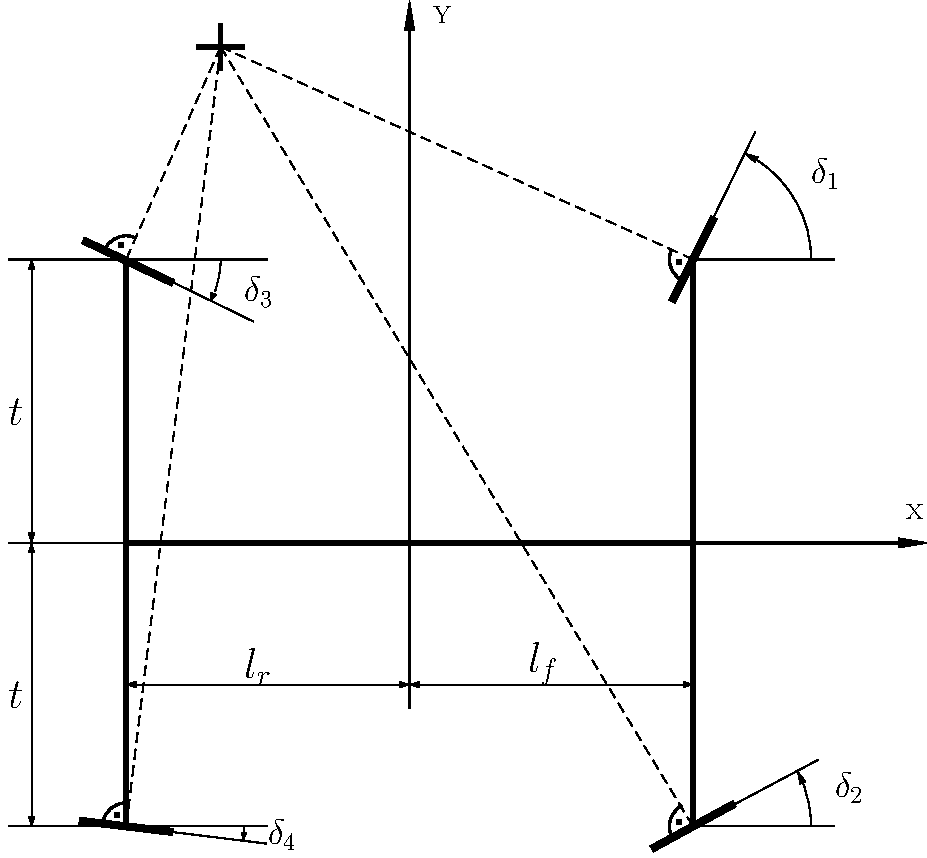
\includegraphics[scale=0.4]{images/example_fig.pdf}
	\end{center}
	\caption[Caption in list of figures]{Caption of the figure}
	\label{fig:figurelabel}
\end{figure}	

\lipsum[2]

\begin{equation}\label{eq:DCmot}
U(t) = Ri(t) + L\cdot\frac{di(t)}{dt} + C\omega(t)
\end{equation}

Pokud máme model popsaný rovnicí \ref{eq:LS_model}, kde \boldmath $\hat{y}$ je odhad výstupu modelu, $b = \left[b_1,b_2,...,b_n\right]^T$ jsou parametry modelu a $X = \left[x_1,x_2,...,x_n\right]$ jsou vstupy modelu, \unboldmath

\begin{center}
	\begin{tabular}{ll}
%		\hline 
		&  \\ 
%		\hline 
		a & 787 \\ 
%		\hline 
		b & 788 \\ 
%		\hline 
		d & 77575 \\ 
%		\hline 
		gf & 7 \\ 
%		\hline 
		h & 6 \\ 
%		\hline 
		hrf & 7 \\ 
%		\hline 
	\end{tabular} 
\end{center}


\begin{equation}\label{eq:LS_model}
\hat{y} = \bm{X} \bm{b}
\end{equation}

\section{Example section}
\label{sec:Example-section}

\begin{equation}\label{eq:DCmot2}
U(t) = Ri(t) + L\cdot\frac{di(t)}{dt} + C\omega(t)
\end{equation}


V kapitole \ref{chap:Expample} \textbf{\textit{v sekci}} \ref{sec:Example-subsection} v obrazku \ref{fig:figurelabel} podle rovnice \ref{eq:DCmot} jak je uvedeno v \cite{Blaha}.




\subsection{Example subsection}
\label{sec:Example-subsection}
\lipsum[6]
\lipsum[7]


\begin{table}[!h] % tabulka parametrů Car4
	\begin{center}
		\begin{tabular}{ccc}
				&  &  \\ 
				&  &  \\ 
				&  &  \\ 
				&  & 

		\end{tabular}
	\end{center}
	\caption[Kratky popisek tabulky]{Popisek Tabulky \cite{Atkeson1996}}
	\label{tab:car4Param}
\end{table}


\lipsum

\begin{figure}[!ht] 
	\begin{center}
		%		\includegraphics[width=\textwidth]{images/LLM_init.pdf}
	\end{center}
	\caption[Kratky popisek]{Popisek obrázku}
	\label{fig:LLM_init}
\end{figure}

\chapter*{Seznam zkratek a symbolů}
\label{chap:loa}
\begin{itemize}
	\item[\textbf{ABS}] Anti-Lock Break System
	
	\item[\textbf{ASR}] Anti-Slip Regulation
	
	\item[\textbf{Car4}] Experimentální vozidlo se čtyřmi hnanými i řízenými koly
	
	\item[\textbf{DOF}] Degree of freedom, Stupeň volnosti
	
	\item[\textbf{ESP}] Electronic Stability Program
	
	\item[\textbf{FSI}] Fakulta strojního inženýrství
\end{itemize}

\chapter*{Seznam příloh} % vlozi kapitolu 2
%\chapter*{List of Abbreviations}
\addcontentsline{toc}{chapter}{List of Abbreviations}
\label{chap:abb}

\begin{itemize}[leftmargin=2.7cm]
	\item[\textbf{LWL}] Locally Weighted Learning
	\item[\textbf{LS}] Least Squares Method
	\item[\textbf{RLS}] Recursive Least Squares Method
	\item[\textbf{RFWR}] Receptive Field Weighted Regression
	\item[\textbf{LOLIMOT}] Local Linear Model Tree
	\item[\textbf{EGR}] Exhaust Gas Recirculation
	\item[\textbf{PID}] Proportional-Integrational-Derivative controller
	
	
\end{itemize}
 % vlozi zkratky

%%%%%%%%%%%%%%%%%%%%%%%%%%%%%%%%%%%%%%%%%%%%%%%%%%%%%%%%%%%%%%%%%%%%%%%%

% \pagestyle{plain}
% \ifthenelse{\equal{\docmode}{print}}
% {
% 	%\fancyhead[LE,RO]{Appendix}
% 	\fancyhead[LO,RE]{Bib}
% 	\fancyfoot[RO]{\thepage}
% 	\fancyfoot[LE]{\thepage}
% }{
% 	%\fancyhead[L]{Appendix}
% 	\fancyhead[R]{Bib}
% 	\fancyfoot[C]{\thepage}
% }
% \begin{thebibliography}{14}
	
	\bibitem{Nellesc2001}
	NELLES, Oliver. \textit{Nonlinear system identification: from classical approaches to neural networks and fuzzy models}. New York: Springer, c2001. ISBN 35-406-7369-5.
	
	\bibitem{Englert2012}
	ENGLERT, Peter. \textit{Locally Weighted Learning} [online]. Darmstadt, Germany, 2012, , 9 [cit. 2016-04-28]. Dostupné z: http://www.ausy.informatik.tu-darmstadt.de/uploads/Teaching/AutonomousLearningSystems/Englert\_ALS\_2012.pdf
	
	\bibitem{Birattari1999}
	BIRATTARI, Mauro a Gianluca BONTEMPI. \textit{The Lazy Learning Toolbox} [online]. 1999, , 30 [cit. 2016-04-28]. DOI: 10.1.1.45.3853. Dostupné z: http://citeseerx.ist.psu.edu/viewdoc/summary?doi=10.1.1.45.3853
	
	\bibitem{Grepl2010}
	GREPL, Robert. Adaptive composite control of electronic throttle using local learning method. In: \textit{2010 IEEE International Symposium on Industrial Electronics} [online]. Brno, the Czech Republic: IEEE, 2010, s.~58-61 [cit. 2016-04-28]. DOI: 10.1109/ISIE.2010.5637899. ISBN 9781424463909. Dostupné z: http://ieeexplore.ieee.org/lpdocs/epic03/wrapper.htm?arnumber=5637899
	
	\bibitem{Zhao2005}
	ZHAO, Y. a J.A. FARRELL. A Locally Weighted Learning Method for Online Approximation Based Control. In: \textit{Proceedings of the 44th IEEE Conference on Decision and Control} [online]. Seville, Spain: IEEE, 2005, s.~2694-2701 [cit. 2016-04-28]. DOI: 10.1109/CDC.2005.1582570. ISBN 0780395670. Dostupné z: http://ieeexplore.ieee.org/lpdocs/epic03/wrapper.htm?arnumber=1582570
	
	\bibitem{Su2004}
	SU, J., J. WANG a Y. XI. Incremental Learning With Balanced Update on Receptive Fields for Multi-Sensor Data Fusion. \textit{IEEE Transactions on Systems, Man and Cybernetics, Part B (Cybernetics)} [online]. 2004, \textbf{34}(1), 659-665 [cit. 2016-04-28]. DOI: 10.1109/TSMCB.2002.806485. ISSN 10834419. Dostupné z: http://ieeexplore.ieee.org/lpdocs/epic03/wrapper.htm?arnumber=1262536
	
	\bibitem{Nakanishi2005}
	NAKANISHI, Jun, Jay A. FARRELL a Stefan SCHAAL. Composite adaptive control with locally weighted statistical learning. \textit{Neural Networks} [online]. 2005, \textbf{18}(1), 71-90 [cit. 2016-04-28]. DOI: 10.1016/j.neunet.2004.08.009. ISSN 08936080. Dostupné z: http://linkinghub.elsevier.com/retrieve/pii/S0893608004001728
	
	\bibitem{Schaal2002}
	SCHAAL, Stefan, Christopher G. ATKESON a Sethu VIJAYAKUMAR. Scalable techniques from nonparametric statistics for real time robot learning. \textit{Applied Intelligence} [online]. 2002, \textbf{17}(1), 49-60 [cit. 2016-04-28]. DOI: 10.1023/A:1015727715131. ISSN 0924669x. Dostupné z: http://link.springer.com/10.1023/A:1015727715131
	
	\bibitem{Vijayakumar2005}
	VIJAYAKUMAR, Sethu, Aaron D'SOUZA a Stefan SCHAAL. Incremental Online Learning in High Dimensions. \textit{Neural Computation} [online]. 2005, \textbf{17}(12), 2602-2634 [cit. 2016-04-28]. DOI: 10.1162/089976605774320557. ISSN 08997667. Dostupné z: http://www.mitpressjournals.org/doi/abs/10.1162/089976605774320557
	
	\bibitem{fpVZRMErpJok1G9j}
	Local dimensionality reduction. SCHAAL, S., S. VIJAYAKUMAR a C.G. ATKESON. \textit{Advances in neural information processing systems 10: proceedings of the 1997 conference ; [presented at the Eleventh Annual Conference on Neural Information Processing (NIPS), held in Denver, Colorado from December 1 to December 6, 1997]} [online]. Electronic version. Cambridge, Mass. [u.a.]: MIT Press, 1998, s.~633-639 [cit. 2016-04-28]. ISBN 0262100762. Dostupné z: http://papers.nips.cc/paper/1387-local-dimensionality-reduction.pdf
	
	\bibitem{Atkeson1997}
	ATKESON, Christopher G., Andrew W. MOORE a Stefan SCHAAL. Locally weighted learning for control. \textit{Artificial Intelligence Review} [online]. 1997, \textbf{11}(1/5), 75-113 [cit. 2016-04-28]. DOI: 10.1023/A:1006511328852. ISSN 02692821. Dostupné z: http://link.springer.com/10.1023/A:1006511328852
	
	\bibitem{Schaal1998}
	SCHAAL, Stefan a Christopher G. ATKESON. Constructive Incremental Learning from Only Local Information. \textit{Neural Computation} [online]. 1998, \textbf{10}(8), 2047-2084 [cit. 2016-04-28]. DOI: 10.1162/089976698300016963. ISSN 08997667. Dostupné z:https://pdfs.semanticscholar.org/0d1d/0b6e29e3b7d6b357537b9e1908b852a37a0e.pdf
	
	\bibitem{Atkeson1996}
	ATKESON, Christopher G., Andrew W. MOORE a Stefan SCHAAL. Locally weighted learning. \textit{Artificial Intelligence Review} [online]. 1996, \textbf{11}(1/5), 11-73 [cit. 2016-04-28]. DOI: 10.1023/A:1006559212014. ISSN 02692821. Dostupné z: http://link.springer.com/10.1023/A:1006559212014
	
	\bibitem{Nakanishi2005}
	NAKANISHI, Jun, Jay A. FARRELL a Stefan SCHAAL. Composite adaptive control with locally weighted statistical learning. \textit{Neural Networks} [online]. 2005, \textbf{18}(1), 71-90 [cit. 2016-05-11]. DOI: 10.1016/j.neunet.2004.08.009. ISSN 08936080. Dostupné z: http://linkinghub.elsevier.com/retrieve/pii/S0893608004001728
	
\end{thebibliography} % vlozi citace
% \ifthenelse{\equal{\docmode}{print}}
% {
% 	%\fancyhead[LE,RO]{Appendix}
% 	\fancyhead[LO,RE]{Bib}
% 	\fancyfoot[RO]{\thepage}
% 	\fancyfoot[LE]{\thepage}
% }{
% 	%\fancyhead[L]{Appendix}
% 	\fancyhead[R]{Bib}
% 	\fancyfoot[C]{\thepage}
% }
% \label{MyLastPage}

% \chapter*{Appendix} % prilohy
% \addcontentsline{toc}{chapter}{Appendix}


% \pagestyle{plain}
% \ifthenelse{\equal{\docmode}{print}}
% {
% 	%\fancyhead[LE,RO]{Appendix}
% 	\fancyhead[LO,RE]{Appendix}
% 	\fancyfoot[RO]{\thepage}
% 	\fancyfoot[LE]{\thepage}
% }{
% 	%\fancyhead[L]{Appendix}
% 	\fancyhead[R]{Appendix}
% 	\fancyfoot[C]{\thepage}
% }


% \lipsum[1]
% \begin{figure}[!h] 
% % * <martin.appel@mechlab.cz> 2018-05-23T10:35:59.125Z:
% %
% % ^.
% 	\begin{center}
% 		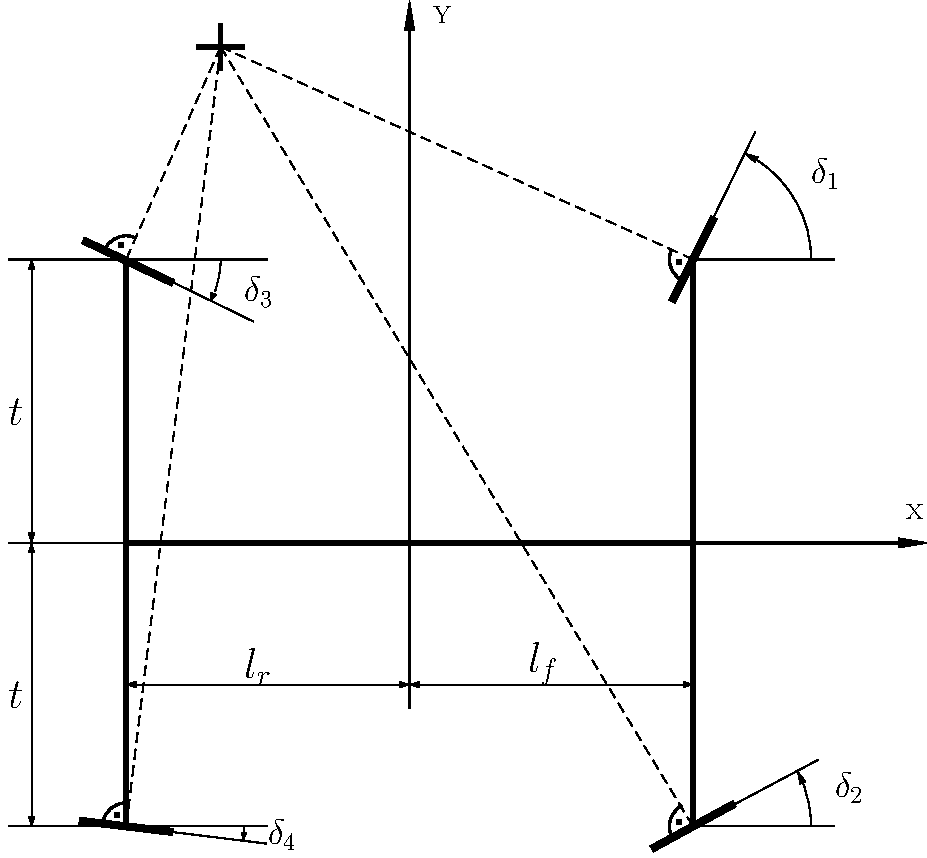
\includegraphics[scale=0.4]{images/example_fig.pdf}
% 	\end{center}
% 	\caption[Caption in list of figures]{Caption of the figure}
% 	\label{fig:figurelabel}
% \end{figure}
% \lipsum[1]
% \begin{figure}[!h] 
% 	\begin{center}
% 		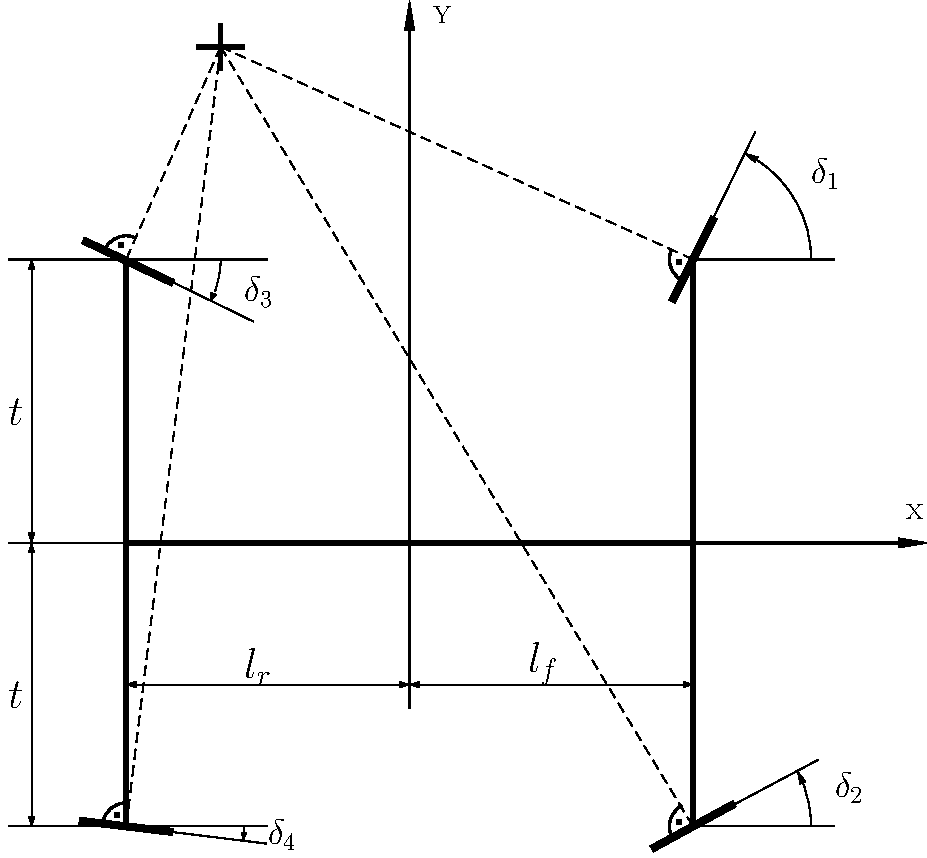
\includegraphics[scale=0.4]{images/example_fig.pdf}
% 	\end{center}
% 	\caption[Caption in list of figures]{Caption of the figure}
% 	\label{fig:figurelabel}
% \end{figure}
% \lipsum[1]
% \begin{figure}[!h] 
% 	\begin{center}
% 		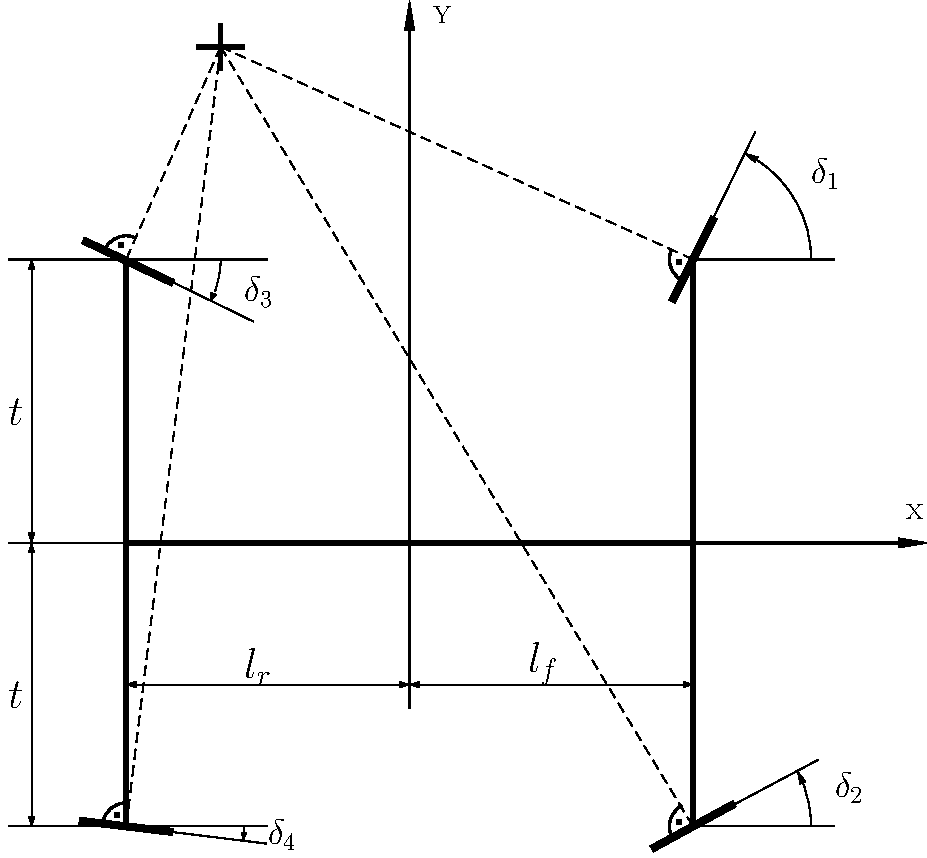
\includegraphics[scale=0.4]{images/example_fig.pdf}
% 	\end{center}
% 	\caption[Caption in list of figures]{Caption of the figure}
% 	\label{fig:figurelabel}
% \end{figure}
% \lipsum[1]
% \begin{figure}[!h] 
% 	\begin{center}
% 		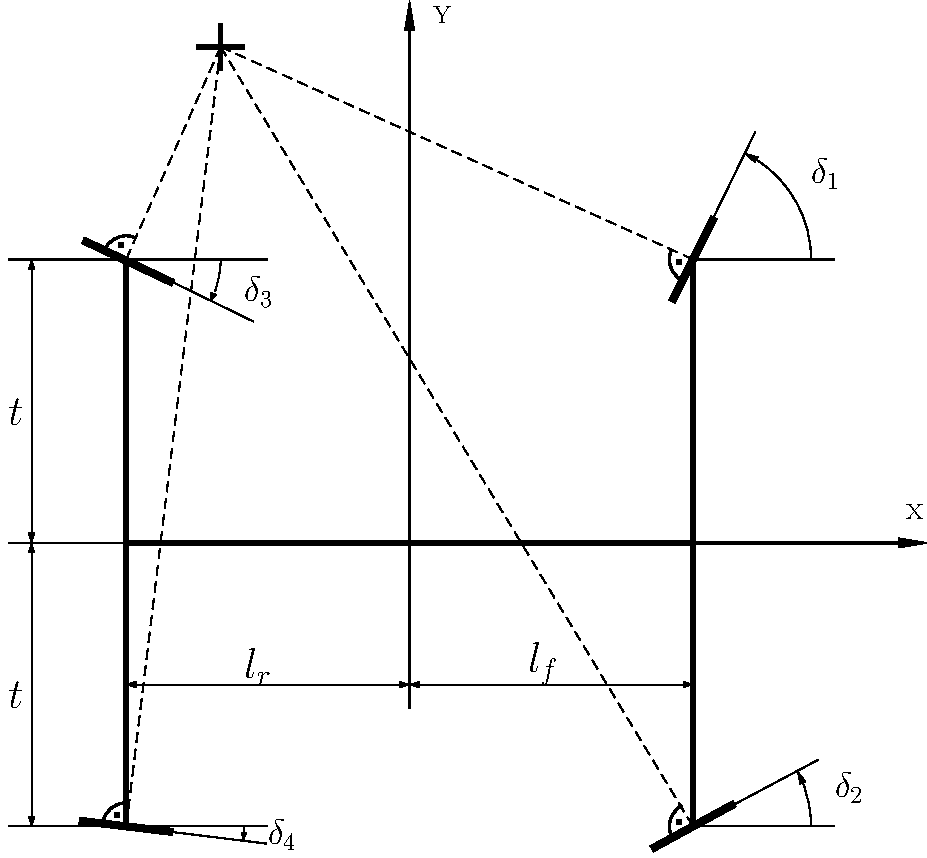
\includegraphics[scale=0.4]{images/example_fig.pdf}
% 	\end{center}
% 	\caption[Caption in list of figures]{Caption of the figure}
% 	\label{fig:figurelabel}
% \end{figure}
% \lipsum[1]
% \begin{figure}[!h] 
% 	\begin{center}
% 		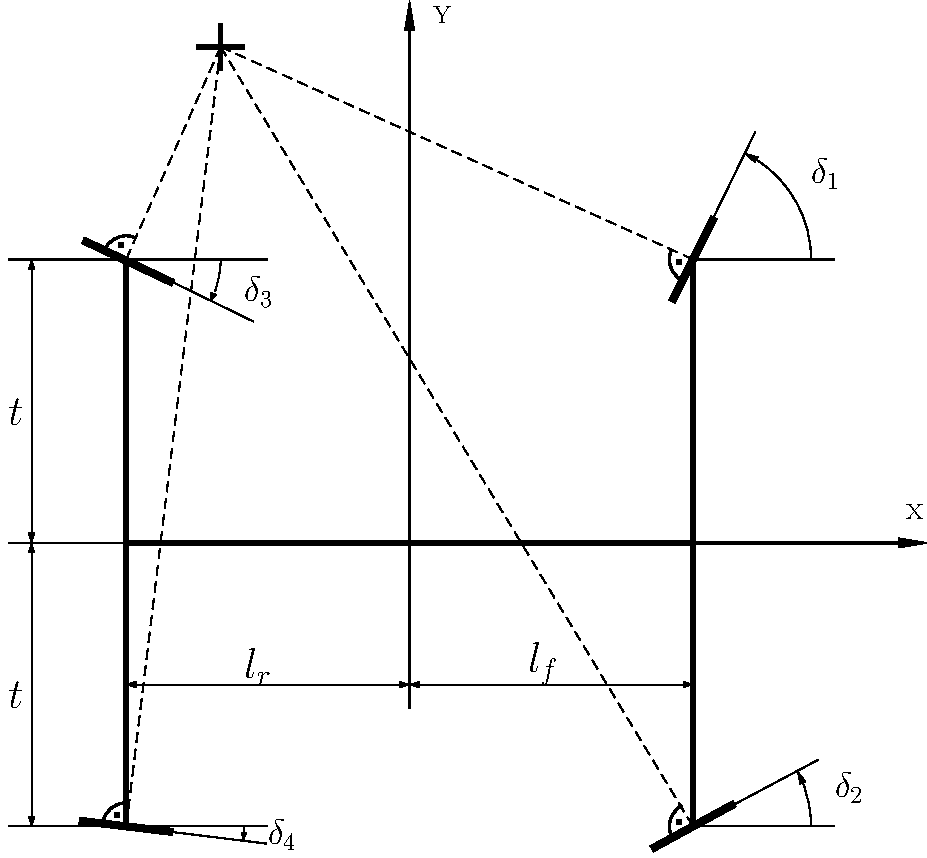
\includegraphics[scale=0.4]{images/example_fig.pdf}
% 	\end{center}
% 	\caption[Caption in list of figures]{Caption of the figure}
% 	\label{fig:figurelabel}
% \end{figure}
% \lipsum[1]
% \begin{figure}[!h] 
% 	\begin{center}
% 		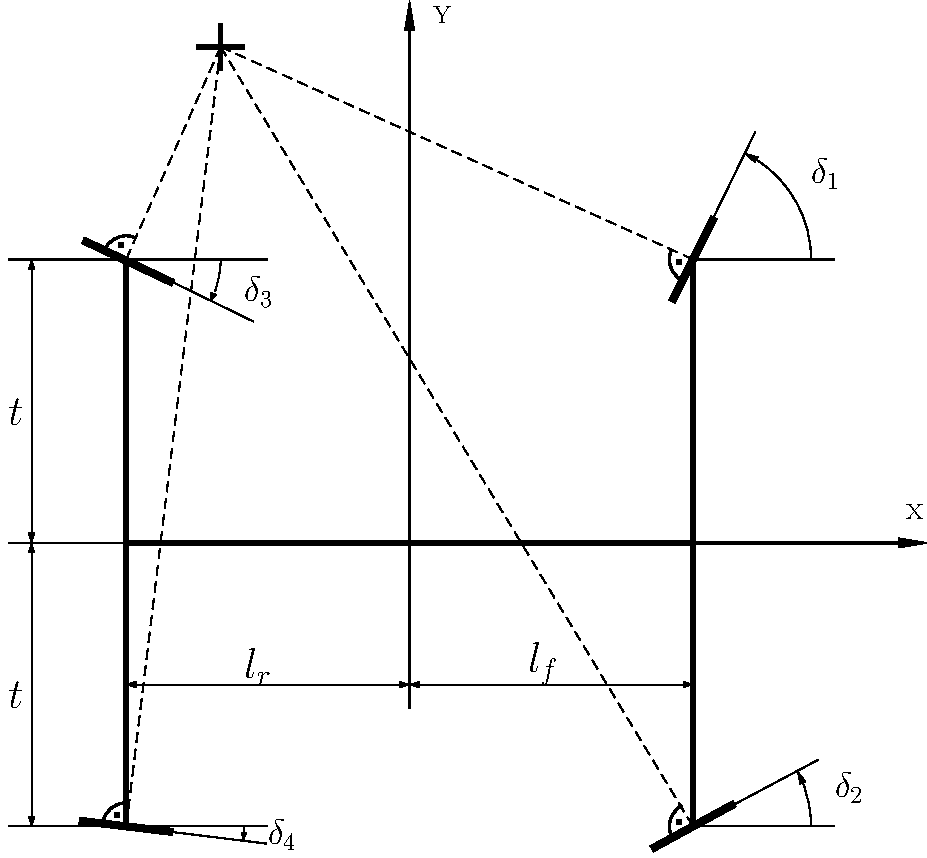
\includegraphics[scale=0.4]{images/example_fig.pdf}
% 	\end{center}
% 	\caption[Caption in list of figures]{Caption of the figure}
% 	\label{fig:figurelabel}
% \end{figure}
% \lipsum[1]
% \begin{figure}[!h] 
% 	\begin{center}
% 		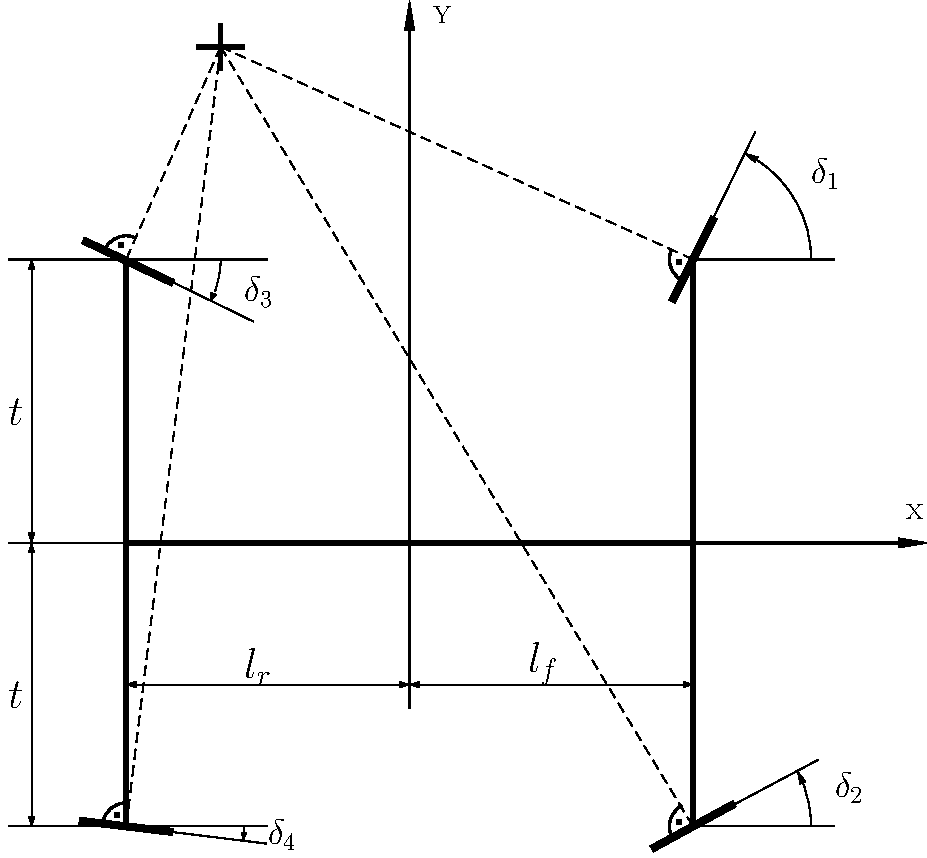
\includegraphics[scale=0.4]{images/example_fig.pdf}
% 	\end{center}
% 	\caption[Caption in list of figures]{Caption of the figure}
% 	\label{fig:figurelabel}
% \end{figure}	


\end{document}